%Dies ist die Hauptseite des Dokumentes. Es werden u. a. alle Kapitel,
%Einstellung im Header eingebunden.  Veränderungen müssen in folgenden Dateien
%vorgenommen werden:
      %- config.tex
      %- einzelne Kapitel (evtl. erweitern)

%Hier sind alle Einstellungen enthalten, die sich auf das Seiten- und
%Dokumentenlayout beziehen

\documentclass[
  11pt,                   % Schriftgröße
  DIV12,
  german,                 % für Umlaute, Silbentrennung etc.
  oneside,                % einseitiges Dokument
  titlepage,              % es wird eine Titelseite verwendet
  parskip=half,           % Abstand zwischen Absätzen (halbe Zeile)
  headings=normal,        % Größe der Überschriften verkleinern
  captions=tableheading,  % Beschriftung von Tabellen unterhalb ausgeben
  final                   % Status des Dokuments (final/draft)
]{scrreprt}               %


%------Ändern von Schriftschnitten - (Muss ganz am Anfang stehen !) ------------
\usepackage{fix-cm}


%------Umlaute -----------------------------------------------------------------
%   Umlaute/Sonderzeichen wie äüöß können direkt im Quelltext verwenden werden.
%    Erlaubt automatische Trennung von Worten mit Umlauten.
\usepackage[T1]{fontenc}
\usepackage[utf8]{inputenc}

%------Anpassung der Landessprache----------------------------------------------
\usepackage[ngerman]{babel}

%------Einfache Definition der Zeilenabstände und Seitenränder------------------
\usepackage{geometry}
\usepackage{setspace}

%------Schriftgrößenanpassung von einzelnen Textpassagen------------------------
\usepackage{relsize}

%------Trennlinien in Kopf- und Fusszeile
\usepackage[headsepline, footsepline, ilines]{scrpage2}

%------Grafiken und Farben -----------------------------------------------------
\usepackage{xcolor}
\usepackage{graphicx}

%------Packet zum Sperren, Unterstreichen und Hervorheben von Texten------------
\usepackage{soul}

%------ergänzende Schriftart----------------------------------------------------
\usepackage{helvet}

%------Lange Tabellen-----------------------------------------------------------
\usepackage{longtable}
\usepackage{array}
\usepackage{ragged2e}
\usepackage{lscape}

%------PDF-Optionen-------------------------------------------------------------
\usepackage[
  bookmarks,
  bookmarksopen=true,
  colorlinks=true,
  linkcolor=black,        % einfache interne Verknüpfungen
  anchorcolor=black,      % Ankertext
  citecolor=black,        % Verweise auf Literaturverzeichniseinträge im Text
  filecolor=black,        % Verknüpfungen, die lokale Dateien öffnen
  menucolor=black,        % Acrobat-Menüpunkte
  urlcolor=black,         % Farbe für URL-Links
  backref,                % Zurücktext nach jedem Bibliografie-Eintrag als
                          % Liste von Überschriftsnummern
  pagebackref,            % Zurücktext nach jedem Bibliografie-Eintrag als
                          % Liste von Seitenzahlen
  plainpages=false,       % zur korrekten Erstellung der Bookmarks
  pdfpagelabels,          % zur korrekten Erstellung der Bookmarks
  hypertexnames=false,    % zur korrekten Erstellung der Bookmarks
  linktocpage             % Seitenzahlen anstatt Text im Inhaltsverzeichnis verlinken
  ]{hyperref}






      % enthält eingebundene Packete

%------Seitenränder-------------------------------------------------------------
\geometry{verbose,                     % zeigt die eingestellten Parameter beim
                                       % Latexlauf an
      paper=a4paper,                   % Papierformat
      top=25mm,                        % Rand oben
      left=25mm,                       % Rand links
      right=25mm,                      % Rand rechts
      bottom=45mm,                     % Rand unten
      pdftex                           % schreibt das Papierformat in die
                                       % Ausgabe damit Ausgabeprogramm
                                       % Papiergröße erkennt
  }

%Seitenlayout
\onehalfspace        % 1,5-facher Abstand

%------Kopf- und Fußzeilen -----------------------------------------------------
\pagestyle{scrheadings}

%------Kopf- und Fußzeile auch auf Kapitelanfangsseiten ------------------------
\renewcommand*{\chapterpagestyle}{scrheadings}

%------Schriftform der Kopfzeile -----------------------------------------------
\renewcommand{\headfont}{\normalfont}

%----Spezielle Befehle
\newcommand{\lfk}[1]{$\langle LF#1\rangle$}

%----Farben
\definecolor{tubsRed}{cmyk}{0.1,1.0,0.8,0.0}
\definecolor{tuRed}{cmyk}{0.1,1.0,0.8,0.0}

%------Kopfzeile----------------------------------------------------------------
\setheadsepline{1pt}[\color{tuRed}]
\setlength{\headheight}{21mm}        % Höhe der Kopfzeile
\ihead{\large{\textsc{\praktikumTitel}}\\    % Text in der linken Box
       \small{\projektTitel}}
\chead{}                            % Text in der mittleren Box

%----Fusszeile
\setfootsepline{1pt}[\color{tuRed}]
\cfoot{}                            % Text in mittlerer Box
\ofoot{\pagemark}                    % Seitenzahl in rechter Box



%------Labels mit eigenem Text für \ref ----------------------------------------
\makeatletter
\def\namedlabel#1#2{\begingroup
#2%
\def\@currentlabel{#2}%
\phantomsection\label{#1}\endgroup
}
\makeatother


%------Neue Environments -------------------------------------------------------

\newcommand{\refsetcounter}[2]{\setcounter{#1}{#2}\addtocounter{#1}{-1}\refstepcounter{#1}}

%Funktion im Pflichtenheft
\newcounter{functioncount} 
\newenvironment{function}[2]{\refsetcounter{functioncount}{#1}\large\textbf{\sffamily{#2 }}\namedlabel{F#1}{$\langle F#1\rangle$}\normalsize\begin{description}\setlength{\itemsep}{-5pt}}{\end{description}}

%Daten im Pflichtenheft
\newcounter{datacount} 
\newenvironment{data}[2]{\refsetcounter{datacount}{#1}\textbf{#2} \namedlabel{D#1}{$\langle D#1\rangle$}\\}{}

%Kriterien im Pflichtenheft
\newcounter{mustcount} 
\newcommand{\must}[2]{\refsetcounter{mustcount}{#1}\namedlabel{RM#1}{$\langle RM#1\rangle$} #2\\}

\newcommand{\should}[2]{\refsetcounter{datacount}{#1}\namedlabel{RS#1}{$\langle RS#1\rangle$} #2\\}

\newcommand{\could}[2]{\refsetcounter{datacount}{#1}\namedlabel{RC#1}{$\langle RC#1\rangle$} #2\\}

\newcommand{\wont}[2]{\refsetcounter{datacount}{#1}\namedlabel{RW#1}{$\langle RW#1\rangle$} #2\\}

%Qualitätsanforderungen im Pflichtenheft
\newcommand{\qualityReq}[2]{\refsetcounter{datacount}{#1}\namedlabel{Q#1}{$\langle Q#1\rangle$} #2\\}

% Benutzeroberflächen im Pflichtenheft
\newcounter{uicount}
\newenvironment{ui}[2]{\refsetcounter{uicount}{#1}\textbf{#2} \namedlabel{UI#1}{$\langle UI#1\rangle$}\\}{}

% Klassen
\newcounter{classcount}
\newenvironment{class}[2]{\refsetcounter{classcount}{#1}\textbf{#2}\namedlabel{CL#1}{$\langle CL#1\rangle$}\begin{description}\setlength{\itemsep}{-5pt}}{\end{description}}

% Entitäten
\newcounter{entitycount}
\newenvironment{entity}[2]{\refsetcounter{entitycount}{#1}\textbf{#2} \namedlabel{E#1}{$\langle E#1\rangle$}\\}{}

% Component
\newcounter{componentcount}
\newenvironment{component}[2]{\refsetcounter{componentcount}{#1}\textbf{Komponente \namedlabel{C#1}{$\langle C#1\rangle$}: #2}\\}{}

% Interface
\newcounter{interfacecount}
\newenvironment{interface}[2]{\refsetcounter{interfacecount}{#1}\textbf{Schnittstelle \namedlabel{I#1}{$\langle I#1\rangle$}: #2}\\}{}

% Testfall
\newcounter{testcasecount}
\newenvironment{testcase}[2]{\clearpage\refsetcounter{testcasecount}{#1}\subsection{Testfall $\langle T#1\rangle$ - #2}\label{T#1}\begin{description}\setlength{\itemsep}{-5pt}}{\end{description}}
           % Diese Datei enthält alle
                                           % Layouteinstellungen
\newcommand{\dokumentTitel}{User instructions}
% Definition von globalen Parametern, die derzeit auf der Titelseite und in der
% Kopfzeile verwendet werden. Der in <> gesetzte Text ist zu verändern.

\newcommand{\praktikumTitel}{SeaCucumber-Framework}
\newcommand{\projektTitel}{for Neo4j}
\newcommand{\institut}{
	Institut für Informationssysteme\\
	Prof. Dr. Wolf-Tilo Balke\\
	Mühlenpfordtstr. 23\\
	38106 Braunschweig\\
}
\newcommand{\institutsLogo}{common/ifis_logo_farbe.pdf}
\newcommand{\betreuer}{Jan-Christoph Kalo, Stephan Mennicke}
\usepackage{listings}
\usepackage{color}

\lstset{%frame=tb,
	language=Java,
	aboveskip=3mm,
	belowskip=3mm,
	showstringspaces=false,
	columns=flexible,
	basicstyle={\small\ttfamily},
	numbers=none,
	numberstyle=\tiny\color{gray},
	keywordstyle=\color{blue},
	commentstyle=\color{dkgreen},
	breaklines=true,
	breakatwhitespace=true,
	tabsize=4
}

%------Beginn des Gesamtdokumentes----------------------------------------------
\begin{document}

%------Eingebundene Seiten, Verzeichnisse bzw. Kapitel--------------------------
% Dies ist die Titelseite.
% Die Ausgabe darf 1 Seite nicht überschreiten, also ggf. Abstände anpassen
% Die Angabe in [...] gibt den Abstand nach der entsprechenden Zeile an.


%----Stil dieser Seite----------------------------------------------------------
\thispagestyle{plain}      % Kopfzeile bleibt leer

%----Beginn der Titelseite------------------------------------------------------
\begin{titlepage}

%----eingebundenes Logo der TU--------------------------------------------------
%\setlength{\unitlength}{1mm}
%  \begin{picture}(00,00)(+25,-04)
%  	\color{tuRed}
%    \put(055,006){\line(1,0){150}}
%    \put(005,000){
\includegraphics[width=6.3cm]{common/TUBraunschweig_4C.pdf}}
%    \put(150,010){\includegraphics[width=8cm,height=2.4cm,keepaspectratio]{\institutsLogo}}
%  \end{picture}\\[5ex]
%\hspace*{-2cm}


\vspace*{-3.8cm}
\hspace*{-2cm}\begin{minipage}{1.25\textwidth}

\includegraphics[width=6.3cm]{common/TUBraunschweig_4C.pdf}\setlength{\unitlength}{1mm}\begin{picture}(00,00)(0,0)\color{tuRed}\put(000,004){\line(1,0){150}}\end{picture}%\hfill
\parbox[b]{0.68\textwidth}{\hfill\includegraphics[width=8cm,height=2.4cm,keepaspectratio]{\institutsLogo}\\~}
\end{minipage}


~\\[5ex]

%----zentrierte Ausrichtung über die gesamte Seite----------------------------
\begin{center}

%----Titel des Praktikum (\praktikumTitel in newComments zu verändern)--------
{\relsize{4}{\textbf{\textsc{\praktikumTitel}}}}\\[5ex]

%----Titel des Teilprojektes (\projektTitel in newComments verändern)---------
{\relsize{3}{\textbf{\textsc{\projektTitel}}}}\\[5ex]

\includegraphics[width=3.5cm]{common/Jar_idee3_3-01.eps}\setlength{\unitlength}{1mm}

Bachelor - Teamprojekt\\
Wintersemester 2017-\the\year\\[6ex]

{\relsize{3}{\textbf{\dokumentTitel}}}\\[5ex]

%----Daten des Auftraggebers
%Auftraggeber\\
%Technische Universität Braunschweig\\
%\institut[2ex]
Betreuer: \betreuer\\[5ex]

%Auftragnehmer: Stephan Mennicke\\

% ----Tabelle der Praktikumsteilnehmer------------------------------------------
\begin{tabular}{l<{\hspace{20mm}} l<{\hspace{30mm}}}\\
  Name                   &   E-Mail-Adresse\\      % Zeilenüberschift

  \hline                    % Linie unterhalb der Zeilenüberschrift
Christian Goldapp & c.goldapp@tu-braunschweig.de\\
Fabian Kirchner & fabian.kirchner@tu-bs.de\\
Maximilian Jahn & maximilian.jahn@tu-bs.de\\
Felix Scholz & felix.scholz@tu-bs.de\\
Maximilian von Unwerth & maximilian.von-unwerth@tu-bs.de\\
Tim Witschel & tim.witschel@tu-bs.de\\

\end{tabular}

%Zur Vereinheitlichung sollten hier die TU Braunschweig Emailadressen benutzt werden. % enthält Tabelle der Praktikumsteilnehmer

\vfill
Braunschweig, \today

\end{center}
\end{titlepage}
                       % Titelseite

%----Bearbeiterübersicht--------------------
%Diese Tabelle ist eine Übersicht, wer welche Teile des Dokumentes verfasst hat. 
%Sie ist vollständig zu bearbeiten.

%\tableofcontents                           % Inhaltsverzeichnis wird automatisch
\setcounter{footnote}{0}   

%----Kapitel des Feinentwurfs, die mit Inhalt zu füllen sind--------------------
\chapter{Instructions}\label{chap:zielbestimmung}
\pagenumbering{arabic}
Dear user,\\
we are delighted that you use our Framework for Neo4j. For everything to run accordingly, you need Neo4j, Maven and Java for our functions and it runs on every operating system that these technologies support.
If you have any questions, please do not hesitate to contact us on our \glqq Git Repository\grqq{}.

\section{Desktop Version} \label{sec:desktop}
If you are using the desktop version, you have to take the following steps. For older Versions see chapter \ref{chap:olderVersion}.

\section{Required-Software}\label{sec:neededsoftwareNew}
In order to use our Framework you need:
\begin{itemize}
	\item The Neo4J-Desktop Client\footnote{\url{https://neo4j.com/download/}}; it has to be installed otherwise you can't run the framework.
	\item The latest version of Java\footnote{\url{https://java.com/de/download/}} has to be installed and the needed root-settings have to be set.
	\item Also your device needs Maven\footnote{\url{https://maven.apache.org/download.cgi}}, this is needed to build the project and import alle dependencies{}.
\end{itemize}
For a better programming experience we recommend to use an IDE. During the instructive steps we use IntelliJ IDEA\footnote{\url{https://www.jetbrains.com/idea/download}}. If you really need this instruction, you should download IntelliJ IDEA and you can install the Framework step by step (See point \ref{sec:stepByStepManualNew} Step by Step Manual).

\newpage

\section {First use guidance for experienced users} \label{sec:beforeFirstUseNew}
\begin{itemize}
	\item The required software should be installed on your computer so you can ensure that everything works correctly.
	\item Start the Neo4j-Desktop Software and create a new database. Instructions are on the Neo4J website.
	\item Now clone our \glqq Git Repository\footnote{\url{https://github.com/vonunwerth/Seacucumber.git}} \grqq{}. If you don't know how to clone the \glqq Git Repository\grqq{} please read the Step by Step Manual.
	\item Furthermore you need to open the project with Maven. You can check your individual IDE for further instructions.
	\item In the package \glqq matcher\grqq{} you can create a new Java class where you implement your algorithm.
	\item The necessary changes to this class, so that \glqq Neo4j - procedures\grqq{} can work properly, will be explained in chapter \ref{sec:startProgrammingNew} \glqq Start coding\grqq{}.
\end{itemize}

\section{Step by step guide for beginners}\label{sec:stepByStepManualNew}
This step by step guide is created for using the software \glqq ItelliJ IDEA\grqq{}.
\begin{itemize}
	\item The requested software should be installed on your computer.
	\item Start the Neo4j-Desktop Software and create a new project (The tab with the book). A new Database can be create with a click on New Graph on the right site. Neo4j will guide you through the creation process. Please take Database Version 3.3.3 \footnote{constituted on 08.03.2018}.
	\item After downloading and installing the Software \glqq IntelliJ IDEA\grqq{} opens and is ready for use. The following window opens. \newpage
	\begin{center}
		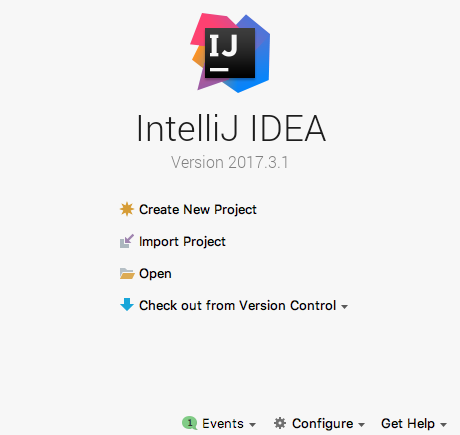
\includegraphics[width=4.2cm]{common/IntelliJstart.png}\setlength{\unitlength}{1mm}
	\end{center}
	
	\item Click on \glqq Check out from Version Control - GitHub\grqq{} and a window with the name \glqq Clone Repository\grqq{} will open. \\
	\textbf{Git Repository URL:} https://github.com/vonunwerth/Seacucumber.git \\
	\textbf{Parent Directory:} The location where you want to save the project.  \\
	\textbf{Directory Name:} For example Neo4j (You can choose whatever you want.)\\
	\\
	Click on Clone and IntelliJ will start to download the repository.
	
	\item You get a at the right corner a notification to add the project as a Maven-project. If the notification doesn't appear look up the trouble shoot chapter \ref{chap:trouble}.
	
	\item All folders should be visible now. Open the src/main/java folder.
	\item In the \glqq package matcher\grqq{} you can create a new Java file to create your algorithm.
\end{itemize}

\section{Start coding}\label{sec:startProgrammingNew}
After checking out the repository you can start coding. Ensure you use Java JDK 1.8 or higher to compile the project. Otherwise some features of the given classes cannot be used.
\begin{itemize}
	\item Create a new class for your new Matching-Algorithm in the matcher package and let your new class extends the abstract class \textit{matcher}.
	\item Implement the \textit{matchingAlgorithm()-method} and import \textit{org.neo4j.graphdb} in order to use the Nodes of Neo4J. Also import the java.util.List instead of the suggested Scala list. Last import java.util.Map to get a result map of your keys and lists of nodes in the end.
	\lstset{language=Java}
	\begin{lstlisting} 
	@Override
	public Map<Integer, List<Node>> matchingAlgorithm() {
	//Your own matcher
	}
	\end{lstlisting} 
	
	\item You have to write a constructor in your class. The constructor's name has to be the same as the classname. The following structure can be used: 
	\lstset{language=Java}
	\begin{lstlisting}
	public [AlgorithmsName] (org.neo4j.graphdb.GraphDatabaseService db, graph.Graph graph) {
	this.db = db; //Describes your database
	this.graph = graph; //Describes your graph
	}
	\end{lstlisting}
	%\begin{center}
	%	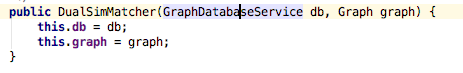
\includegraphics[width=10.5cm]{common/MatcherConstrutor.png}\setlength{\unitlength}{1mm}
	%\end{center}
	A lot of prewritten methods can be found in the abstract \glqq Matcher\grqq{} class. Check our javadoc for more information.
	\item Now you have to create a now procedure to access your matcher on your Neo4J database. Go to the \textit{procedure.GraphProcedures} class and e.g. copy one of the example procedures for Dual Simulation or Failures.
	\begin{lstlisting}
	@Procedure(value = "graph.[NAME]", mode = Mode.READ)
	@Description("[DESCRIPTION]")
	@SuppressWarnings("unused")
	public Stream<NodeResult> [NAME](@Name("query") String 	query) {
	Graph graph = prepareQuery(db, query);
	[MATCHER] matcher = new [MATCHER](db, graph);
	Set<Node> simulated = matcher.simulate();
	return simulated.stream().map(NodeResult::new);
	}
	\end{lstlisting} 
	Replace [NAME] with the name of your new procedure and [MATCHER] with the name of your new matcher class.
\end{itemize}

\section{After coding}\label{sec:afterProgrammingNew}
After you write your algorithm in your new class in the Java package matcher, you have to create the \glqq jar\grqq{} for the database.
\begin{itemize}
	\item Before you create the jar, you can test the code. Please use the \glqq ProcedureTest\grqq{} class in the test package. For testing start the main method in the class \glqq ProcedureTest.java\grqq{}.
	\item Open the Maven tab in \glqq IntelliJ \grqq{} and open the point \glqq Neo4JMatchAlgFramework\grqq{}. The next folder you need is the \glqq Lifecycle\grqq{} folder, here you click \glqq clean\grqq{} then you click on \glqq package\grqq{}.
	\item After finishing you start your explorer and search for the folder where you cloned the \glqq Git Repository\grqq{} to. Here is a new folder named target. Open this folder and copy the \glqq original-Neo4JMatchAlgFramework-1.0.jar\grqq{}. \\
	(The other one is for testing and is not important. It won't work.)
	\item Please go to your Neo4j database from the first steps (see step by step manual \ref{sec:stepByStepManualNew}).
	You must paste the \glqq Neo4JMatchAlgFramework-1.0.jar\grqq{} to the \glqq plugins\grqq{} Folder. 
	\\The \glqq plugins\grqq{} Folder can be find after click on the \glqq Manage\grqq{} button at the database tab. Then click on open Folder and you will see the \glqq plugins\grqq{} Folder. 
	\item After doing this you can call your procedure in Neo4j. If you are ready, start the database with the Neo4j software.
\end{itemize}

\section{Work with Neo4j}\label{sec:takeneo4jNew}
To test if your procedure works in Neo4j you can use the following example statements.
\begin{itemize}
	\item You want to use your procedures? Then use the CALL-Statement.\\
	For example:
	\begin{lstlisting}
	CALL graph.exampleQuery(
	"MATCH (m:Movie)<-[:DIRECTED]-(p:Person) 
	RETURN m,p")
	\end{lstlisting}
	\item You want to take your procedures and would like to search with another query on this result? Then take the CALL statement and the YIELD statement. \\
	For example:
	
	\begin{lstlisting}
	CALL graph.exampleQuery(
	"MATCH (m:Movie)<-[:DIRECTED]-(p:Person)
	RETURN m,p") 
	YIELD node MATCH (m:Movie)<-[:DIRECTED]-(p:Person)
	RETURN m,p
	\end{lstlisting}
\end{itemize}
At this point you know everything we know - have fun and develop new algorithms.
\newpage

\chapter{For older Versions} \label{chap:olderVersion}
If you use older versions (Neo4j Community Edition 3.2.6), the steps are not the same as the steps at the Neo4j-Desktop version.

\section{Required-Software}\label{sec:neededsoftware}
In order to use our Framework you need:
\begin{itemize}
	\item The Neo4J Client\footnote{\url{https://neo4j.com/download/other-releases/\#releases}} is very important; it has to be installed otherwise you can't run the framework.
	\item The latest version of Java\footnote{\url{https://java.com/de/download/}} has to be installed and the needed root-settings have to be set.
	\item Also your device needs Maven\footnote{\url{https://maven.apache.org/download.cgi}}, this is needed to build the project and import alle dependencies{}.
\end{itemize}
For a better programming experience we recommend to use an IDE. During the instructive steps we use IntelliJ IDEA\footnote{\url{https://www.jetbrains.com/idea/download}}. If you really need this instruction, you should download IntelliJ IDEA and you can install the Framework step by step (See point \ref{sec:stepByStepManual} Step by Step Manual).

\newpage

\section {First use guidance for experienced users} \label{sec:beforeFirstUse}
\begin{itemize}
	\item The required Software should be installed on your computer so you can ensure that everything works right.
	\item Please start the Neo4j - Software and create a new database. 
	\item The plugin folder has to be created in the following directory(neo4j/default.graphdb/plugins). You need this for your \glqq  Neo4j - Procedures\grqq{}.
	\item Now you need our Framework. You can clone our \glqq Git Repository\footnote{\url{https://github.com/vonunwerth/Seacucumber.git}} \grqq{}. If you don't now how to clone the \glqq Git Repository\grqq{} please read the Step by Step Manual.
	\item Furthermore you need to open the project with Maven. You can check your individual IDE for further instructions.
	\item In the package \glqq matcher\grqq{} you can create a new Java class where you implement your algorithm.
	\item Things that need to be changed in this class, so that \glqq Neo4j - procedures\grqq{} can work properly, will be explained in chapter \ref{sec:startProgramming} \glqq Start coding\grqq{}. 
\end{itemize}

\section{Step by step guide for beginners}\label{sec:stepByStepManual}
This step by step guide is created for using the software \glqq ItelliJ IDEA\grqq{}.
\begin{itemize}
	\item The requested Software should be installed on your computer.
	\item Please start the Neo4j - Software and create a new database. Neo4j will guide you through the creation process. One important thing is to know where the databse is stored. (By default the folder is called neo4j/default.graphdb). \\(Nice to know for login: by default the username and password is neo4j)
	\item The plugin folder has to be created in the following directory(neo4j/default.graphdb/plugins). You need this for your \glqq  Neo4j - Procedures\grqq{}.
	\newpage
	\item After downloading and installing the Software \glqq IntelliJ IDEA\grqq{} opens and is ready for use. The following window opens. \\
	\begin{center}
		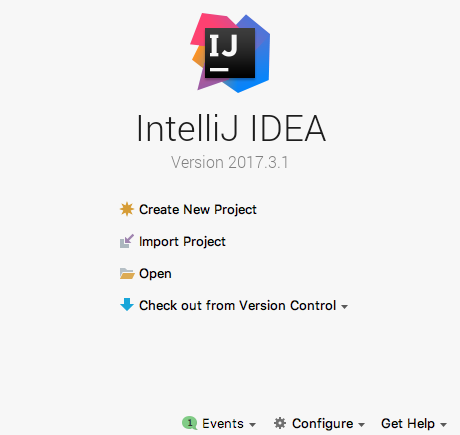
\includegraphics[width=4.2cm]{common/IntelliJstart.png}\setlength{\unitlength}{1mm}
	\end{center}
	
	\item You click on \glqq Check out from Version Control - GitHub\grqq{} and a window with the name \glqq Clone Repository\grqq{} will open. \\
	\textbf{Git Repository URL:} https://github.com/vonunwerth/Seacucumber.git \\
	\textbf{Parent Directory:} The location where you want to save the project.  \\
	\textbf{Directory Name:} For example Neo4j (You can choose whatever you want.)\\
	\\
	Click on Clone and IntelliJ will start to download the repository.
	
	\item You get a at the right corner a notification to add the project as a Maven-project. If the notification doesn't appear look up the trouble shoot chapter \ref{chap:trouble}.
	
	\item All folders should be visible now. Open the src/main/java folder.
	\item In the \glqq package matcher\grqq{} you can create a new Java file to create your algorithm.
\end{itemize}

\section{Start coding}\label{sec:startProgramming}
After checking out the repository you can start coding. Ensure you use Java JDK 1.8 or higher to compile the project. Otherwise some features of the given classes cannot be used. It's the same steps like the newer Versions. Please see section \ref{sec:startProgrammingNew}.

\section{After coding}\label{sec:afterProgramming}
After you write your algorithm in your new class in the Java package matcher, you have to create the \glqq jar\grqq{} for the database.
\begin{itemize}
	\item Before you create the jar, you can test the code. Please use the \glqq ProcedureTest\grqq{} class in the test package. For testing start the main method in the class \glqq ProcedureTest.java\grqq{}.
	\item Open the Maven tab in \glqq ItelliJ \grqq{} and open the point \glqq Neo4JMatchAlgFramework\grqq{}. The next folder you need is the \glqq Lifecycle\grqq{} folder, here you click \glqq clean\grqq{} then you click on \glqq package\grqq{}.
	\item After finishing you start your explorer and search for the folder where you cloned the \glqq Git Repository\grqq{} to. Here is a new folder named target. Open this folder and copy the \glqq original-Neo4JMatchAlgFramework-1.0.jar\grqq{}. \\
	(The other one is for testing and is not important. It won't work.)
	\item Please go to your Neo4j database from the first steps (see step by step manual).%felix
	You must paste the \glqq Neo4JMatchAlgFramework-1.0.jar\grqq{} to the previously created \glqq plugins\grqq{} Folder.
	\item After doing this you can call your procedure in Neo4j. If you are ready, start the database with the Neo4j software.
\end{itemize}

\section{Work with Neo4j}\label{sec:takeneo4j}
To test if your procedure works in Neo4j you can use the following example statements.
\begin{itemize}
	\item You want to use your procedures? Then use the CALL-Statement.\\
	For example:
	\begin{lstlisting}
	CALL graph.exampleQuery(
	"MATCH (m:Movie)<-[:DIRECTED]-(p:Person) 
	RETURN m,p")
	\end{lstlisting}
	\item You want to take your procedures and would like to search with another query on this result? Then take the CALL statement and the YIELD statement. \\
	For example:
	
	\begin{lstlisting}
	CALL graph.exampleQuery(
	"MATCH (m:Movie)<-[:DIRECTED]-(p:Person)
	RETURN m,p") 
	YIELD node MATCH (m:Movie)<-[:DIRECTED]-(p:Person)
	RETURN m,p
	\end{lstlisting}
\end{itemize}
At this point you know everything we know - So have fun and develop new good algorithms.
\newpage

\chapter{Trouble shooting} \label{chap:trouble}

\begin{itemize}
	\item 
		The Folder with our \glqq Git Repository\grqq{} is displayed at the \glqq IntelliJ\grqq{} window, but you only see \glqq readme\grqq{}and other data but not the Java files. \\
		If you want see the Java files, open the Maven Tab on the right side. Click on the tab and on the circle on the left corner. You will be ask, if you want to \glqq import Maven Projects\grqq{} - click \glqq yes\grqq{}. The \glqq Maven Dependencies\grqq{} are now downloaded, this needs a while.
		\begin{center}
			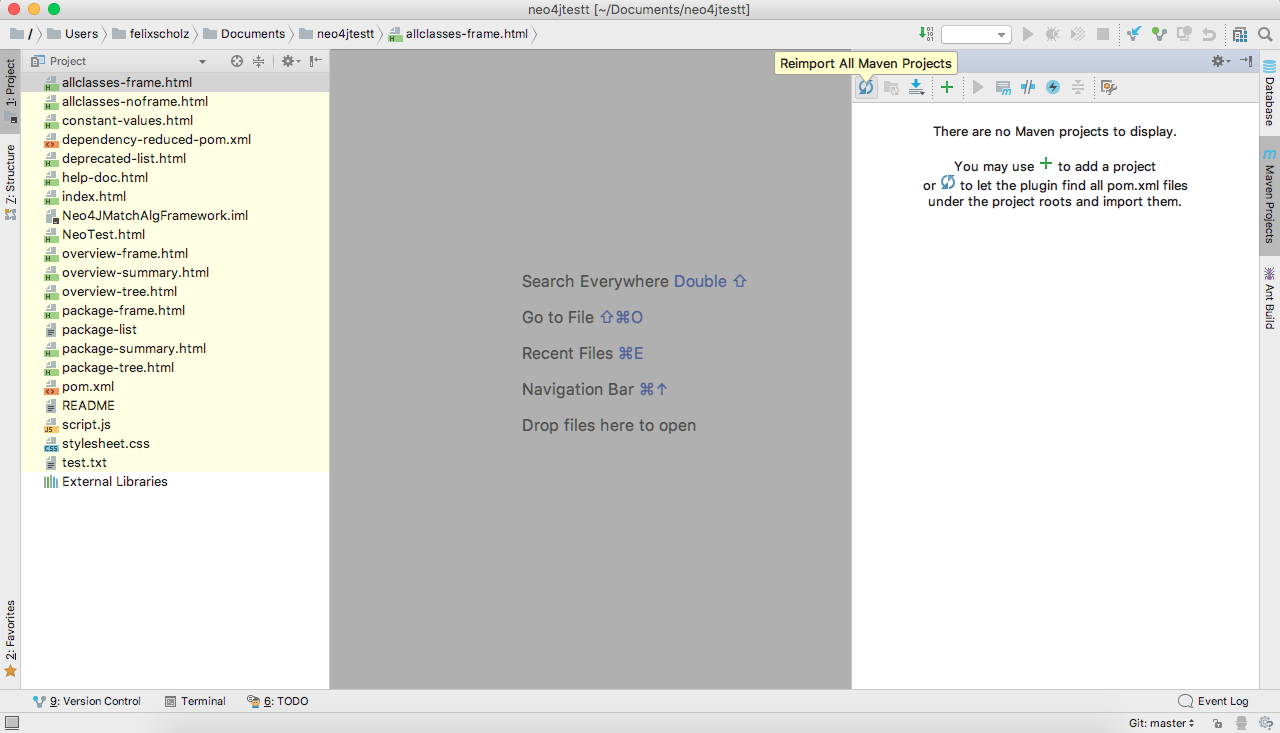
\includegraphics[width=10.3cm]{common/MavenImport.png}\setlength{\unitlength}{1mm}
		\end{center}
\end{itemize}

%\include{Pflichtenheft/01_zielbestimmung}
%\include{Pflichtenheft/02_produkteinsatz}
%\include{Pflichtenheft/03_produktuebersicht}
%\include{Pflichtenheft/04_produktfunktionen}
%\include{Pflichtenheft/05_produktdaten}
%\include{Pflichtenheft/06_nichtfunktionaleanforderungen}
%\include{Pflichtenheft/07_benutzeroberflaeche}
%\include{Pflichtenheft/08_produktumgebung}
%\include{Pflichtenheft/09_glossar}

%------Ende des Dokumentes------------------------------------------------------
\end{document}
